% !TEX program = lualatex
% !TEX encoding = UTF-8
\documentclass[12pt,aspectratio=169]{beamer}

\usepackage{luatexja}
\usepackage{amsmath, amssymb, bm}
\usepackage{physics}
\usepackage{tikz}
\usepackage{xcolor}
\usepackage{appendixnumberbeamer}
\usetikzlibrary{arrows.meta, positioning, shapes}

\usetheme{Madrid}
\usecolortheme{seahorse}
\setbeamertemplate{navigation symbols}{}

\definecolor{myblue}{RGB}{30, 80, 160}
\definecolor{myred}{RGB}{180, 40, 40}
\definecolor{mygreen}{RGB}{30, 130, 60}

\title[TD-gGA]{時間依存ゴースト Gutzwiller 近似\\
  \large (Time-dependent ghost Gutzwiller Approximation)}
\subtitle{Guerci, Capone, Lanat\`a, PRR \textbf{5}, L032023 (2023)}
\author{東川 喜斗}
\institute{埼玉大学}
\date{\today}

\begin{document}

% ============================================================
\begin{frame}
  \titlepage
\end{frame}

% ============================================================
\begin{frame}{目次}
  \begin{enumerate}\itemsep10pt
    \item \textbf{概要}\\
      {\small 動機・手法比較・DMFT・平衡ベンチマーク}
    \item \textbf{静的 gGA}\\
      {\small 変分波動関数・埋め込みH・自己無撞着条件}
    \item \textbf{TD-gGA}\\
      {\small クエンチ設定・運動方程式・主要結果}
    \item \textbf{まとめ}
  \end{enumerate}
\end{frame}

% ============================================================
\begin{frame}[plain]
  \vfill
  \centering
  {\usebeamercolor[fg]{structure}\Large\textbf{I. 概要}}\\[8pt]
  {\small 動機・手法比較・DMFT・平衡ベンチマーク}
  \vfill
\end{frame}

% ============================================================
\begin{frame}{なぜ非平衡ダイナミクスか？}
  \begin{columns}[T]
    \begin{column}{0.50\textwidth}
      \textbf{強相関電子系の非平衡物性：}
      \begin{itemize}
        \item Mott 絶縁体，Kondo 効果，高温超伝導…\\
          \textcolor{myblue}{平衡理論は大きく発展}
        \item 非平衡・時間依存の問題は\\
          \textcolor{myred}{理論的に難しく未解明な点が多い}
      \end{itemize}

      \medskip
      \begin{alertblock}{中心的な問い}
        相互作用を\textbf{突然変化}させると\\
        量子系はどう応答・緩和するか？
      \end{alertblock}
    \end{column}

    \begin{column}{0.47\textwidth}
      \textbf{実験的動機：}
      \begin{block}{超冷却原子 $+$ 光格子}
        \small
        Feshbach 共鳴で $U$ を人為的・\\
        瞬時に変化させられる\\
        $\to$ クエンチの\textbf{理想的な実験台}
      \end{block}

      \smallskip
      \begin{block}{フェムト秒ポンプ-プローブ}
        \small
        固体中の Mott 状態を光パルスで\\
        叩き，超高速緩和を時間分解観測
      \end{block}

      \smallskip
      {\small $\Rightarrow$ クエンチダイナミクスを定量的に計算できる理論が必要}
    \end{column}
  \end{columns}
\end{frame}

% ============================================================
\begin{frame}[shrink=5]{DMFT のアイデア：格子問題 $\to$ Anderson 不純物}
  \begin{columns}[T]
    \begin{column}{0.50\textwidth}
      \textbf{DMFT の発想：}
      \begin{itemize}
        \item 格子の多体問題を\textbf{単一サイト問題}に帰着
        \item 各サイト $\longleftrightarrow$ Anderson 不純物 + bath（自己無撞着）
      \end{itemize}

      \begin{block}{\small 正当化：$d\to\infty$ 極限}
        \small
        配位数 $z\to\infty$ で自己エネルギーが局所的に：\\
        $\Sigma(\mathbf{k},\omega) \to \Sigma(\omega)$\\
        $\Rightarrow$ 格子問題が単一サイト問題に等価に帰着\\
        {\footnotesize （Metzner-Vollhardt 1989）}
      \end{block}

      \smallskip
      \begin{block}{gGA の発想}
        \small
        DMFT の bath（連続的な混成関数 $\Delta(\omega)$）を\\
        \textbf{$B$ 個の ghost 軌道}で変分的に近似する
      \end{block}

      \smallskip
      \begin{alertblock}{時間依存の問題}
        \small
        TD-DMFT：bath の記憶効果 $\to$ 積分微分方程式
      \end{alertblock}
    \end{column}

    \begin{column}{0.47\textwidth}
      \textbf{自己無撞着ループ：}
      \smallskip
      \begin{tikzpicture}[scale=0.78,
          box/.style={draw,rounded corners,text width=3.2cm,
                      align=center,inner sep=4pt,font=\footnotesize}]
        \node[box,draw=myblue,fill=myblue!6](d) at (0,4.0)
          {$\Delta(\omega)$ を初期推定};
        \node[box,draw=myred,fill=myred!8](imp) at (0,2.6)
          {不純物モデルを解く\\{\tiny CTQMC など（高コスト）}};
        \node[box](sig) at (0,1.2)
          {$\Sigma(\omega)$ を抽出};
        \node[box](g) at (0,-0.1)
          {$G_\mathrm{lattice}(\omega)$ を計算};
        \node[box,draw=myblue,fill=myblue!6](dn) at (0,-1.3)
          {新しい $\Delta(\omega)$ を抽出};
        \draw[->,thick](d)--(imp);
        \draw[->,thick](imp)--(sig);
        \draw[->,thick](sig)--(g);
        \draw[->,thick](g)--(dn);
        \draw[->,thick,myblue](dn.east)--++(0.5,0)
          |-(d.east) node[midway,right,font=\tiny]{収束まで};
      \end{tikzpicture}

      \smallskip
      {\scriptsize
        $\Delta(\omega)$：混成関数（bath との結合の強さ）\\
        \quad cf.\ gGA では $\mathcal{D}_a$（離散化した混成振幅）\\
        $\Sigma(\omega)$：自己エネルギー（相互作用の補正項）\\
        $G_\mathrm{lattice}(\omega)$：格子 Green 関数（相互作用込みの格子の電子伝播）
      }
    \end{column}
  \end{columns}
\end{frame}

% ============================================================
\begin{frame}[shrink=5]{gGA vs DMFT：平衡ベンチマーク}
  \begin{columns}[T]
    \begin{column}{0.50\textwidth}
      \centering
      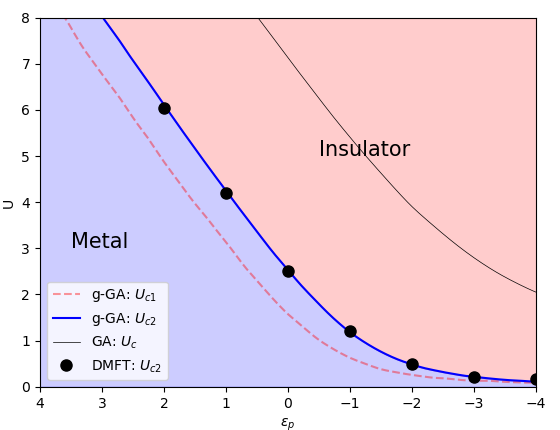
\includegraphics[width=\textwidth]{bench_Figure1.png}
      {\footnotesize Frank \textit{et al.}, \textit{PRB} \textbf{104}, L081103 (2021)\\
      Anderson 格子模型，Bethe 格子}
    \end{column}

    \begin{column}{0.47\textwidth}
      {\small
      \textcolor{myblue}{青線}：gGA $U_{c2}$\quad
      黒点：DMFT\quad
      細黒線：bare GA
      }

      \smallskip
      \begin{block}{\small セッティング}
        \small
        Anderson 格子模型（$p$+$d$），Bethe 格子\\
        $\langle\hat{N}_i\rangle=3$，$V=1$，gGA：$B=3$\\
        DMFT：CTQMC，$T=0.01$\\
        コスト：gGA $\sim$0.2秒 vs DMFT $\sim$2分（72コア）
      \end{block}

      \medskip
      \begin{alertblock}{\small 結論}
        \small \textbf{gGA ($B=3$) は DMFT と驚くべき一致}\\
        bare GA は $\varepsilon_p\ll -1$ で大きくずれる
      \end{alertblock}
    \end{column}
  \end{columns}
\end{frame}

% ============================================================
\begin{frame}[shrink=5]{手法の比較：なぜ gGA か}
  \begin{columns}[T]
    \begin{column}{0.48\textwidth}
      \begin{block}{GA（Gutzwiller 近似）}
        \begin{itemize}
          \item 計算コストが低い
          \item \textcolor{myred}{定量的精度に問題あり}\\
            （Mott 転移点・相関効果がずれる）
        \end{itemize}
      \end{block}

      \medskip
      \begin{block}{DMFT}
        \begin{itemize}
          \item 配位数無限で厳密
          \item 強相関系の基準手法
          \item \textcolor{myred}{計算コストが高い}
        \end{itemize}
      \end{block}
    \end{column}

    \begin{column}{0.48\textwidth}
      \begin{alertblock}{今日の主役：gGA}
        \begin{center}
          \textbf{精度} $\approx$ DMFT\\[4pt]
          \textbf{コスト} $\approx$ GA\\[4pt]
          {\small ghost（補助）軌道を導入して\\GA の精度問題を解決}
        \end{center}
      \end{alertblock}

      \medskip
      \centering
      \begin{tikzpicture}[scale=0.82,
          box/.style={draw,rounded corners,text width=2.6cm,
                      align=center,inner sep=4pt}]
        \node[box,draw=myred,fill=myred!6](ga)   at (-1.6,1.0)
          {\small GA\\コスト◎ 精度×};
        \node[box,draw=myred,fill=myred!6](dmft) at ( 1.6,1.0)
          {\small DMFT\\精度◎\\コスト×};
        \node[box,draw=mygreen,fill=mygreen!8](gga) at (-1.6,-1.1)
          {\small\textbf{gGA}\\精度◎\\コスト◎};
        \draw[->,myblue,thick](ga)--(gga)
          node[midway,left,font=\footnotesize]{ghost 軌道};
      \end{tikzpicture}
    \end{column}
  \end{columns}
\end{frame}

% ============================================================
\begin{frame}[plain]
  \vfill
  \centering
  {\usebeamercolor[fg]{structure}\Large\textbf{II. 静的 gGA}}\\[8pt]
  {\small 変分波動関数・埋め込みH・自己無撞着条件}
  \vfill
\end{frame}

% ============================================================
\begin{frame}[shrink=5]{gGA の変分波動関数}
  \begin{columns}[T]
    \begin{column}{0.50\textwidth}
      \textbf{対象：半充填 Hubbard モデル}
      \begin{equation*}
        \hat{H} = \frac{U}{2}\sum_i(\hat{n}_i-1)^2
                  - J\!\sum_{\langle i,j\rangle,\sigma}
                    c^\dagger_{i\sigma}c_{j\sigma}
      \end{equation*}

      \smallskip
      \textbf{変分波動関数：}
      \begin{equation*}
        |\Psi_G\rangle = \hat{\mathcal{P}}_G |\Psi_0\rangle
      \end{equation*}
      \begin{itemize}
        \item $|\Psi_0\rangle$：ghost（補助）空間の Slater 行列式
        \item $\hat{\mathcal{P}}_G$：補助空間 $\to$ 物理空間への線形写像
        \item 各物理サイトに $B$ 個の ghost 軌道
      \end{itemize}

    \end{column}

    \begin{column}{0.47\textwidth}
      \centering
      \begin{tikzpicture}[scale=0.70,
          imp/.style={circle,draw=myred,fill=myred!15,
                      minimum size=24pt,font=\small},
          bath/.style={circle,draw=myblue,fill=myblue!10,
                       minimum size=18pt,font=\footnotesize}]
        \node[imp](c) at (0,0){$c_\sigma$};
        \node[myred,below=4pt of c,font=\footnotesize]{物理サイト};
        \node[bath](f1) at (-1.8,1.8){$f_1$};
        \node[bath](f2) at (0,2.2){$f_2$};
        \node[bath](fB) at (1.8,1.8){$f_B$};
        \node at (0,2.9){\small$\cdots$};
        \draw[myblue,thick](c)--(f1)
          node[midway,left,font=\tiny]{$\mathcal{D}_1$};
        \draw[myblue,thick](c)--(f2);
        \draw[myblue,thick](c)--(fB)
          node[midway,right,font=\tiny]{$\mathcal{D}_B$};
        \node[myblue,font=\scriptsize,below=18pt of c]
          {ghost 軌道（$B$ 個）};
      \end{tikzpicture}

      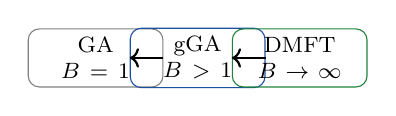
\begin{tikzpicture}[scale=0.72,
          box/.style={draw,rounded corners,text width=1.5cm,
                      align=center,inner sep=3pt,font=\footnotesize}]
        \node[box,draw=gray](ga) at (0,0){GA\\$B=1$};
        \node[box,draw=myblue](gga) at (1.8,0){gGA\\$B>1$};
        \node[box,draw=mygreen](dmft) at (3.6,0){DMFT\\$B\to\infty$};
        \draw[->,thick](ga)--(gga);
        \draw[->,thick](gga)--(dmft);
      \end{tikzpicture}

      \smallskip
      \begin{block}{\small $B$ と精度の対応}
        \small
        \begin{tabular}{cl}
          $B=1$         & 通常の Gutzwiller 近似（GA）\\
          $B=2,3,\ldots$ & 精度が系統的に向上\\
          $B\to\infty$  & DMFT に漸近
        \end{tabular}
      \end{block}
    \end{column}
  \end{columns}
\end{frame}

% ============================================================
\begin{frame}[shrink=5]{埋め込みハミルトニアン（Embedding Hamiltonian）}
  \begin{columns}[T]
    \begin{column}{0.50\textwidth}
      {\footnotesize \textbf{変分原理の帰結：}\\
      エネルギー（作用）を\textbf{最小化}すると，\\
      以下の局所的な有効問題に帰着する．}

      \medskip
      各サイトの局所的有効問題：
      \begin{align*}
        \hat{H}^i_\mathrm{emb}[\mathcal{D}_i,\Lambda^c_i] &=
          \frac{U}{2}(\hat{n}_{c_i}-1)^2\\
          &+\sum_{a,\alpha}\bigl([\mathcal{D}_i]_{a\alpha}\,c^\dagger_{i\alpha} b_{ia}+\mathrm{h.c.}\bigr)\\
          &+\sum_{a,b}[\Lambda^c_i]_{ab}\,b^\dagger_{ia}b_{ib}
      \end{align*}
      \small
      $c^\dagger_{i\alpha}$：物理サイト（軌道 $\alpha$），\ $b_{ia}^\dagger$：ghost bath 軌道\\
      $[\mathcal{D}_i]_{a\alpha}$：結合，\ $[\Lambda^c_i]_{ab}$：bath 内エネルギー

      \smallskip
    \end{column}

    \begin{column}{0.47\textwidth}
      \textbf{準粒子ハミルトニアン（補助空間）：}
      {\small
      \begin{align*}
        \hat{H}_\mathrm{qp}[\mathcal{R},\Lambda] &=
          \sum_{i,j}\sum_{a,b}
          [\mathcal{R}^\dagger J_{ij}\mathcal{R}]_{ab}
          f^\dagger_{ia}f_{jb}\\
          &+\sum_{i}\sum_{a,b}[\Lambda]_{ab}f^\dagger_{ia}f_{ib}
      \end{align*}
      }
      \small
      $\mathcal{R}$：hopping 繰り込み行列\\
      $\Lambda$：準粒子エネルギーへの補正項

      \smallskip
      \begin{block}{\small $\hat{H}^i_\mathrm{emb}$ の次元数}
        \small
        一般：$4^{\nu_i(B+1)}$（$\nu_i$：物理軌道数）\\
        単軌道（$\nu_i=1$）：$4^{B+1}$\\
        \quad $B=3$：256 次元，$B=7$：65536 次元
      \end{block}
    \end{column}
  \end{columns}
\end{frame}

% ============================================================
\begin{frame}[shrink=5]{平衡 gGA：自己無撞着条件}
  \begin{columns}[T]
    \begin{column}{0.52\textwidth}
      Lagrangian の停留条件から：

      \textbf{F1 条件}（$\mathcal{R}$ を局所問題から——Gutzwiller 近似）：
      {\small
      \begin{align*}
        \langle c^\dagger_{i\alpha}b_{ia}\rangle_\mathrm{emb}
          = \sum_c[\Delta_i(1-\Delta_i)]^{\frac{1}{2}}_{ac}[\mathcal{R}_i]_{c\alpha}
      \end{align*}
      }

      \textbf{F2 条件}（bath 占有数の整合性）：
      \begin{equation*}
        \langle b^\dagger_{ia}b_{ib}\rangle_\mathrm{emb}
          = [\Delta_i]_{ab}
          \equiv \langle\Psi_0|f^\dagger_{ia}f_{ib}|\Psi_0\rangle_\mathrm{qp}
      \end{equation*}

      {\small ※ $\Lambda_{ab}$（$\hat{H}_\mathrm{qp}$ 側）は F2 の Lagrange 乗数として自己無撞着に決定，一般に $\Lambda\neq0$}
    \end{column}

    \begin{column}{0.45\textwidth}
      \textbf{自己無撞着ループ：}
      \begin{tikzpicture}[scale=0.78,
          box/.style={draw,rounded corners,text width=2.8cm,
                      align=center,inner sep=4pt,font=\footnotesize}]
        \node[box](start) at (0,5.6){$\mathcal{R}$, $\Lambda$ を初期推定};
        \node[box](delta) at (0,4.0){$\hat{H}_\mathrm{qp}$ を解く\\$\Delta$ を計算};
        \node[box,draw=myblue,fill=myblue!6](update) at (0,2.4){$\mathcal{D}$, $\Lambda^c$ を更新};
        \node[box](emb)   at (0,0.8){$\hat{H}_\mathrm{emb}$ を構築\\基底状態 $|\Phi\rangle$};
        \node[box](check) at (0,-0.8){F1（$\mathcal{R}$ 更新）, F2 を評価};
        \draw[->,thick](start)--(delta);
        \draw[->,thick](delta)--(update);
        \draw[->,thick](update)--(emb);
        \draw[->,thick](emb)--(check);
        \draw[->,thick,myblue](check.east)--++(0.5,0)
          |-(delta.east)
          node[midway,right,font=\tiny]{収束まで};
      \end{tikzpicture}
    \end{column}
  \end{columns}
\end{frame}

% ============================================================
\begin{frame}[plain]
  \vfill
  \centering
  {\usebeamercolor[fg]{structure}\Large\textbf{III. TD-gGA}}\\[8pt]
  {\small クエンチ設定・運動方程式・主要結果}
  \vfill
\end{frame}

% ============================================================
\begin{frame}[shrink=3]{非平衡への拡張：相互作用クエンチ}
  \begin{columns}[T]
    \begin{column}{0.50\textwidth}
      \textbf{ハミルトニアン}（半充填 Hubbard モデル）
      \begin{equation*}
        \hat{H} = \frac{U}{2}\sum_i (\hat{n}_i-1)^2
                  - J\!\sum_{\langle i,j\rangle,\sigma} c^\dagger_{i\sigma}c_{j\sigma}
      \end{equation*}
      \textbf{クエンチ：}$t=0$ で $U_i \to U_f$（突然変化）

      \medskip
      \begin{alertblock}{観測量：二重占有数}
        $d(t)=\langle \hat{n}_{i\uparrow}\hat{n}_{i\downarrow}\rangle$
        ＝同一サイトに $\uparrow\downarrow$ が\textbf{共存する確率}\\[2pt]
        {\small $U\to\infty$（Mott）: $d\to 0$\quad
                $U=0$（非相互作用）: $d=1/4$}\\[2pt]
        $\Rightarrow$ TD-DMFT と同じ量で\textbf{直接比較可能}
      \end{alertblock}

      \smallskip
      {\small Bethe 格子，エネルギー単位 $D$，時間単位 $D^{-1}$}
    \end{column}

    \begin{column}{0.47\textwidth}
      \centering
      \begin{tikzpicture}[scale=0.9]
        \draw[->,thick](-0.3,0)--(4.2,0) node[right]{$t$};
        \draw[->,thick](0,-0.3)--(0,2.5) node[above]{$U(t)$};
        \draw[myblue,very thick](-0.2,0.4)--(1.5,0.4);
        \node[myblue,left,font=\small] at (0,0.4){$U_i$};
        \draw[dashed,gray](1.5,0)--(1.5,2.1);
        \node[below,font=\small] at (1.5,-0.05){$t=0$};
        \draw[myred,very thick](1.5,2.0)--(4.0,2.0);
        \node[myred,right,font=\small] at (4.0,2.0){$U_f$};
        \draw[myred,->,very thick](1.5,0.5)--(1.5,1.9);
        \node[right,font=\small] at (1.6,1.2){クエンチ};
      \end{tikzpicture}

      \smallskip
      \begin{block}{\small gGA を時間依存に拡張}
        \small
        平衡 gGA の低コスト・高精度を\\
        そのまま非平衡ダイナミクスへ
      \end{block}
    \end{column}
  \end{columns}
\end{frame}

% ============================================================
\begin{frame}[shrink=18]{TD-gGA の運動方程式}
  \begin{columns}[T]
    \begin{column}{0.52\textwidth}
      \textbf{Dirac--Frenkel 変分原理：}\\
      {\small $|\Psi_G\rangle$ の形を保ったまま $\hat{H}$ で時間発展させるため，\\
      $|\Psi_G\rangle$ の空間に留まりながら\\
      Schrödinger 方程式に最も近い時間発展を選ぶ}
      \begin{equation*}
        \delta\Bigl\langle\Psi_G(t)\Big|i\partial_t-\hat{H}\Big|\Psi_G(t)\Bigr\rangle=0
      \end{equation*}
      {\scriptsize
        $i\partial_t|\Psi_G\rangle$：変分空間内での実際の発展\\
        $\hat{H}|\Psi_G\rangle$：ハミルトニアンが要求する本来の発展\\
        $\Rightarrow$ 2つの差を\textbf{最小}にする時間発展を選ぶ
      }

      \begin{block}{$\Downarrow$ 適用すると}
        \centering
        \textbf{埋め込みH の Schrödinger 方程式}
        \begin{equation*}
          i\partial_t|\Phi(t)\rangle = \hat{H}_\mathrm{emb}(t)\,|\Phi(t)\rangle
        \end{equation*}
        {\small $\mathcal{R},\mathcal{D},\Delta$ は各時刻で代数的に更新}
      \end{block}
    \end{column}

    \begin{column}{0.45\textwidth}
      \textbf{何が嬉しいか：}
      \begin{itemize}
        \item $\hat{H}_\mathrm{emb}$ は有限次元（$4^{B+1}$）\\
          $\Rightarrow$ Runge--Kutta で\textbf{直接積分可能}
        \item 各時刻で代数的に更新\\
          $\Rightarrow$ 各時刻での\textbf{自己無撞着ループ（反復計算）が不要}
      \end{itemize}

      \medskip
      \begin{tikzpicture}[scale=0.73,
          box/.style={draw,rounded corners,fill=white,
                      text width=3.2cm,align=center,inner sep=4pt,
                      font=\small}]
        \node[box,draw=myred,fill=myred!8](dmft) at (0,0){
          \textbf{TD-DMFT}\\[2pt]
          積分微分方程式\\[1pt]
          \textcolor{myred}{コスト $O(t^2)$}
        };
        \node[right=8pt of dmft,font=\small,text width=4.5cm,myred]
          {
            $\displaystyle \int_0^t \Sigma(t,t') G(t') \, dt'$\\[6pt]
            {\footnotesize 過去の全履歴の積分が必要\\$\to$ 全体コスト $O(t^2)$}\\[4pt]
            {\footnotesize (Aoki \textit{et al.} 2014, App. A)}
          };
        \node[box,draw=mygreen,fill=mygreen!8](gga) at (0,-2.8){
          \textbf{TD-gGA}\\[2pt]
          常微分方程式\\[1pt]
          \textcolor{mygreen}{コスト $O(t)$}
        };
        \draw[->,very thick,myblue](dmft)--(gga);
      \end{tikzpicture}
    \end{column}
  \end{columns}
\end{frame}

% ============================================================
% ============================================================
\begin{frame}[shrink=8]{主要結果：$d(t)$ のクエンチ応答}
  \begin{columns}[T]
    \begin{column}{0.60\textwidth}
      \centering
      \includegraphics[width=\columnwidth]{{fig2(a)}.png}\\
      {\scriptsize Guerci, Capone, Lanat\`a,
        \textit{PRR} \textbf{5}, L032023 (2023) Fig.2(a)}

      \smallskip
      {\scriptsize
        Bethe 格子，半充填，$\Lambda=0$ ゲージ固定\\
        $U_i\simeq0.05$（$U_i=0$ では $\hat{H}_\mathrm{emb}$ が縮退するため）\\
        $B=1,3,5,7$（色で区別），黒点：TD-DMFT（Eckstein et al.）\\
        時間積分：RKSUITE（adaptive Runge-Kutta）\quad
        $\hbar=1$，$D=1$，時間単位 $D^{-1}$
      }
    \end{column}

    \begin{column}{0.37\textwidth}
      \textbf{読み取れること：}
      \begin{itemize}
        \item $B=1$（灰）：永続振動，緩和なし
        \item $B$ を増やすにつれ\\
          DMFT（黒点）の緩和に近づく
        \item $B=7$ で $t\lesssim6$ まで\\
          \textcolor{mygreen}{TD-DMFT とほぼ一致}
      \end{itemize}

      \medskip
      \begin{alertblock}{\small コスト比較}
        \small
        TD-gGA：$O(t)$\\
        TD-DMFT：$O(t^2)$
      \end{alertblock}

    \end{column}
  \end{columns}
\end{frame}

% ============================================================
\begin{frame}[shrink=10]{なぜ ghost bath が緩和を可能にするか}
  \centering
  \includegraphics[width=0.92\textwidth]{{fig2(b)}.png}\\
  {\scriptsize 上段：$\Lambda^c$ の固有値，下段：$\sqrt{\mathcal{D}^\dagger\mathcal{D}}$（$B=7$，各 $\delta U$）\quad
  Guerci et al., \textit{PRR} \textbf{5}, L032023 (2023) Fig.2(b)}

  \vfill
  {\small
  $B\geq3$ で変分空間が豊かになると ghost bath が動的に応答できる\\[3pt]
  \textbf{上段}：bath のエネルギー準位（$\Lambda^c$ 固有値）がクエンチ直後に大きく変動し新たな定常値へ\\
  \textbf{下段}：impurity-bath 結合（$\sqrt{\mathcal{D}^\dagger\mathcal{D}}$）が適応的に変化\\[3pt]
  $\Rightarrow$ bath が動的に応答しているから $d(t)$ の緩和が可能になる
  }
\end{frame}

% ============================================================
\begin{frame}[plain]
  \vfill
  \centering
  {\usebeamercolor[fg]{structure}\Large\textbf{IV. まとめ}}
  \vfill
\end{frame}

% ============================================================
\begin{frame}[shrink=3]{まとめ}
  \begin{columns}[T]
    \begin{column}{0.54\textwidth}
      \begin{block}{TD-gGA の要点}
        \medskip
        \begin{enumerate}\itemsep4pt
          \item \textbf{各サイト} $=$ Anderson 不純物 $+$ $B$ ghost bath
          \item \textbf{埋め込みH}：$4^{B+1}$ 次元の局所問題
          \item \textbf{Dirac--Frenkel 原理} $\to$ 閉じた ODE
          \item \textbf{$\Lambda=0$ 固定}で実装（$\Lambda^c$ は自由発展）
          \item $B=7$ で $t\lesssim6$ まで TD-DMFT とほぼ一致，コスト $O(t)$
        \end{enumerate}
        \medskip
      \end{block}
    \end{column}

    \begin{column}{0.43\textwidth}
      \begin{block}{今後の課題}
        \medskip
        \begin{itemize}\itemsep4pt
          \item 外場 $\mathbf{A}(t)$ を加えた\\
            ダイナミクスの研究\\
            {\footnotesize（ODE なので容易に拡張可能）}
          \item 長時間での熱化の検証
          \item クエンチの強さ $\delta U$ を変えた\\
            ときのダイナミクスの相図の\\
            $B$ 依存性
        \end{itemize}
        \medskip
      \end{block}
    \end{column}
  \end{columns}

  \smallskip
  {\footnotesize
    Guerci, Capone, Lanat\`{a}, \textit{PRR} \textbf{5}, L032023 (2023)\quad
    Lanat\`{a}, \textit{Slave-Boson Theories}, Lect.\ notes (2023)
  }

  \medskip
  \centering\large ご清聴ありがとうございました

\end{frame}

\appendix

% ============================================================
\begin{frame}{付録A：ベンチマーク — モデル設定}
  \textbf{Anderson 格子模型（ALM）ハミルトニアン：}
  \begin{equation*}
    \hat{H} = \sum_{\langle i,j\rangle\sigma}
      \bigl(t_{ij}+\delta_{ij}\varepsilon_p\bigr)
      p^\dagger_{i\sigma}p^{\phantom\dagger}_{j\sigma}
      +\frac{U}{2}\sum_i(\hat{n}_{di}-1)^2
      +V\sum_{i\sigma}
      \bigl(p^\dagger_{i\sigma}d^{\phantom\dagger}_{i\sigma}+\mathrm{h.c.}\bigr)
      -\mu\sum_i\hat{N}_i
  \end{equation*}

  \begin{columns}[T]
    \begin{column}{0.48\textwidth}
      \begin{block}{自由度と軌道}
        \small
        $p_{i\sigma}$：遍歴軌道（非相関）\\
        $d_{i\sigma}$：相関軌道（Hubbard $U$）\\
        $\hat{N}_i = \hat{n}_{pi}+\hat{n}_{di}$，充填：$\langle\hat{N}_i\rangle=3$
      \end{block}
    \end{column}
    \begin{column}{0.48\textwidth}
      \begin{block}{パラメータ}
        \small
        $V=1$（$p$-$d$ 混成，固定），Bethe 格子\\
        $\varepsilon_p$：$p$ 軌道準位（$-4$～$+3$ で変化）\\
        エネルギー単位：$\varepsilon_k$ の半幅（半円型 DOS）
      \end{block}
    \end{column}
  \end{columns}
\end{frame}

% ============================================================
\begin{frame}{付録A：ベンチマーク — 数値計算の詳細}
  \begin{columns}[T]
    \begin{column}{0.48\textwidth}
      \begin{block}{gGA の設定}
        \small
        ghost 軌道数：$B=3$\\
        埋め込みH の次元：$4^{B+1}=64$\\
        Figure 2 の $\varepsilon_p$：$1,\ {-0.5},\ {-2}$
      \end{block}

      \medskip
      \begin{alertblock}{充填条件}
        \small
        $\langle\hat{N}_i\rangle = \langle\hat{n}_{pi}\rangle+\langle\hat{n}_{di}\rangle = 3$\\
        粒子-正孔変換で $\langle N\rangle=1$ の相図も得られる
      \end{alertblock}
    \end{column}

    \begin{column}{0.48\textwidth}
      \begin{block}{DMFT（CTQMC）の設定}
        \small
        温度：$T=0.01$（$\varepsilon_p=-2$ のみ $T=0.02$）\\
        MC ステップ：$5\times10^8$\\
        並列：72 コア，$\sim2$ 分/反復\\
        スペクトル：最大エントロピー法で解析接続
      \end{block}

      \medskip
      \begin{block}{コスト比較}
        \small
        gGA：1 コア，$\sim0.2$ 秒/反復\\
        $\Rightarrow$ DMFT 比 $\sim40000$ 倍高速
      \end{block}
    \end{column}
  \end{columns}
\end{frame}

% ============================================================
\begin{frame}[shrink=5]{付録B：超冷却原子 $+$ 光格子のセットアップ}
  \begin{columns}[T]
    \begin{column}{0.50\textwidth}
      \textbf{実験の流れ：}
      {\small
      \begin{enumerate}\itemsep2pt
        \item 真空チャンバー内に原子気体（例：$^6$Li）を封入
        \item レーザー冷却 $+$ 磁気光学トラップ \hfill $\sim\mu$K
        \item 蒸発冷却（熱い原子を逃がす） \hfill $\sim$nK
        \item 離調レーザー（例：1064 nm）を真空中に向けて照射\\
              定在波 $\to$ 周期ポテンシャル $\to$ 原子が整列
      \end{enumerate}
      }

      \smallskip
      \begin{alertblock}{\small ポイント}
        \small
        固体や基板は一切なし——\\
        \textbf{真空中に浮いた原子}にレーザーをかぶせる\\
        格子欠陥ゼロ，パラメータ完全制御
      \end{alertblock}
    \end{column}

    \begin{column}{0.47\textwidth}
      \textbf{固体 $\leftrightarrow$ 冷却原子の対応：}
      \smallskip

      {\small
      \begin{tabular}{ll}
        \hline
        \textbf{固体} & \textbf{冷却原子} \\
        \hline
        格子点 & 光格子の谷 \\
        電子ホッピング $J$ & 原子トンネリング \\
        & （格子深さで調整）\\
        Coulomb 斥力 $U$ & 接触相互作用 \\
        & （Feshbach で調整）\\
        \hline
      \end{tabular}
      }

      \smallskip
      \begin{block}{\small 格子間隔}
        \small
        $d = \lambda/2 \approx 530$ nm（1064 nm レーザーの場合）\\
        実固体（$\sim$0.3 nm）より $\sim$1000 倍大きいが\\
        無次元比 $U/J$ は同様に調整可能
      \end{block}
    \end{column}
  \end{columns}
\end{frame}

% ============================================================
\begin{frame}[shrink=5]{付録B：超冷却原子によるクエンチの実現}
  \begin{columns}[T]
    \begin{column}{0.52\textwidth}
      \textbf{光格子 $+$ Feshbach 共鳴：}
      \begin{itemize}
        \item 光格子中冷却原子 $=$ フェルミ・Hubbard モデル
        \item $U \propto a$（s波散乱長）
      \end{itemize}

      \smallskip
      \textbf{Feshbach 共鳴のしくみ：}

      \begin{tikzpicture}[scale=0.62]
        \draw[->,thick](0,-0.2)--(0,2.1) node[above]{\small $E$};
        \draw[->,thick](-0.2,0)--(3.8,0) node[right]{\small $B$};
        \draw[myblue,thick](0,1.1)--(3.6,1.1)
          node[right,font=\tiny]{開チャンネル閾値};
        \draw[myred,thick](0,2.0)--(3.6,0.2)
          node[right,font=\tiny]{閉チャンネル};
        \draw[dashed,gray](1.9,0)node[below,font=\tiny]{$B_0$}--(1.9,1.1);
        \fill[mygreen](1.9,1.1) circle(2.5pt);
        \node[mygreen,font=\tiny,right] at (2.0,1.3){共鳴};
      \end{tikzpicture}

      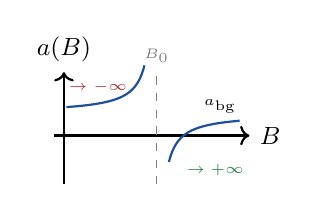
\begin{tikzpicture}[scale=0.62]
        \draw[->,thick](0,-1.0)--(0,1.3) node[above]{\small $a(B)$};
        \draw[->,thick](-0.2,0)--(3.8,0) node[right]{\small $B$};
        \draw[dashed,gray](1.9,-1.0)--(1.9,1.3)
          node[above,font=\tiny]{$B_0$};
        \draw[myblue,thick,domain=0.05:1.65,samples=60]
          plot(\x,{0.45*(1-0.55/(\x-1.9))});
        \draw[myblue,thick,domain=2.15:3.6,samples=60]
          plot(\x,{0.45*(1-0.55/(\x-1.9))});
        \node[font=\tiny] at (3.2,0.6){$a_\mathrm{bg}$};
        \node[myred,font=\tiny] at (0.7,1.0){$\to-\infty$};
        \node[mygreen,font=\tiny] at (3.1,-0.7){$\to+\infty$};
      \end{tikzpicture}
    \end{column}

    \begin{column}{0.45\textwidth}
      \textbf{クエンチの実現：}

      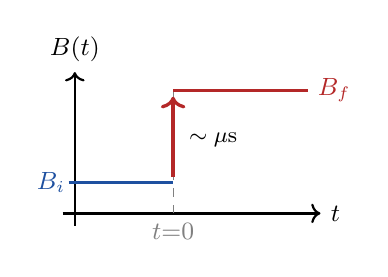
\begin{tikzpicture}[scale=0.78]
        \draw[->,thick](-0.2,0)--(4.0,0) node[right]{\small $t$};
        \draw[->,thick](0,-0.2)--(0,2.3) node[above]{\small $B(t)$};
        \draw[myblue,very thick](-0.1,0.5)--(1.6,0.5);
        \node[myblue,left,font=\small] at (0,0.5){$B_i$};
        \draw[dashed,gray](1.6,0)node[below,font=\small]{$t{=}0$}--(1.6,2.0);
        \draw[myred,very thick](1.6,2.0)--(3.8,2.0);
        \node[myred,right,font=\small] at (3.8,2.0){$B_f$};
        \draw[myred,->,very thick](1.6,0.6)--(1.6,1.9);
        \node[right,font=\footnotesize] at (1.7,1.2){$\sim\mu$s};
      \end{tikzpicture}

      \smallskip
      \begin{block}{\small タイムスケール・観測}
        \small
        磁場スイッチ：$\sim\mu$s，ダイナミクス：$\sim$ms\\
        $\Rightarrow$ スイッチは「瞬時」とみなせる\\[3pt]
        量子気体顕微鏡で $d(t)$ を時間分解観測
      \end{block}
    \end{column}
  \end{columns}
\end{frame}

% ============================================================
\begin{frame}[shrink=15]{付録B：フェムト秒ポンプ-プローブ分光}
  \begin{columns}[T]
    \begin{column}{0.50\textwidth}
      \textbf{実験の仕組み：}

      \begin{tikzpicture}[scale=0.85]
        \node[draw,fill=myblue!10,rounded corners,
              minimum width=1.2cm,minimum height=1.5cm,
              font=\footnotesize] (sample) at (2.2,0) {試料};
        \draw[->,myred,very thick] (0,0.5) -- (1.6,0.1)
          node[midway,above,font=\footnotesize]{ポンプ光};
        \draw[->,myblue,thick] (0,-0.5) -- (1.6,-0.1)
          node[midway,below,font=\footnotesize]{プローブ光};
        \draw[->,mygreen,thick] (2.8,0) -- (4.0,0)
          node[midway,above,font=\footnotesize]{検出};
        \node[font=\tiny,myred] at (0.3,1.0){$\sim100\,\mathrm{fs}$};
        \node[font=\tiny,myblue] at (0.3,-1.1){遅延 $t$};
      \end{tikzpicture}

      \smallskip
      \begin{itemize}
        \item \textbf{ポンプ}：フェムト秒レーザーで電子系を瞬時に励起
        \item \textbf{プローブ}：遅延 $t$ 後に別パルスで状態を観測
        \item 時間分解能：フェムト秒〜アト秒（$10^{-15}$〜$10^{-18}$ s）
      \end{itemize}

      \smallskip
      \begin{block}{\small 非平衡との関係}
        \small
        ポンプで突然エネルギーを注入\\
        $\Rightarrow$ クエンチに近い状況（ただし $U$ が\\
        変わるわけではなく光励起が主体）
      \end{block}
    \end{column}

    \begin{column}{0.47\textwidth}
      \textbf{観測される現象（光誘起相転移）：}
      \begin{itemize}
        \item 光誘起絶縁体—金属転移
        \item 光誘起中性—イオン性転移
        \item 超高速磁性ダイナミクス
        \item ペタヘルツ固体スイッチ
      \end{itemize}

      \smallskip
      \begin{block}{\small タイムスケール}
        \small
        パルス幅：$\sim100\,\mathrm{fs}$\\
        エネルギー密度：温度換算で $10^4$ K 相当\\
        $\Rightarrow$ 少数の光子で多数の原子・分子を変化
      \end{block}

      \smallskip
      \begin{block}{\small 参考}
        \small
        岡本博，「強相関電子系の超高速光誘起相転移」\\
        \textit{物性研究} \textbf{1}(0), 176 (2014)\\[2pt]
        「光誘起相転移の挑戦」\\
        \textit{日本物理学会誌} \textbf{71}(6) (2016)\\[2pt]
        岩井研究室（東北大）\url{femto.phys.tohoku.ac.jp}
      \end{block}
    \end{column}
  \end{columns}
\end{frame}

% ============================================================
\begin{frame}[shrink=8]{付録C：gGA vs DMFT — $Z$・エネルギーの収束（3軌道 Hubbard）}
  \begin{columns}[T]
    \begin{column}{0.48\textwidth}
      \centering
      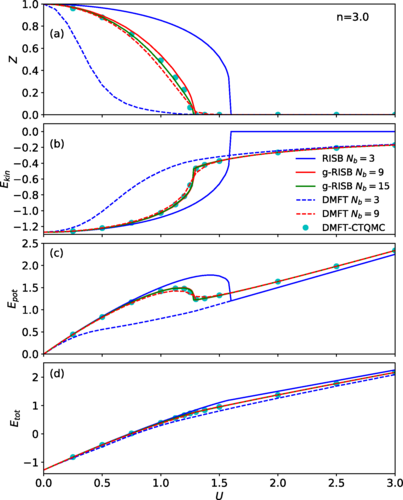
\includegraphics[width=0.70\textwidth]{hub_fig3.png}
    \end{column}
    \begin{column}{0.48\textwidth}
      \small
      3軌道 Hubbard モデル，Bethe 格子\\
      $n=3$（半充填），$J=0.25U$

      \smallskip
      \begin{block}{\small 凡例}
        \footnotesize
        青実線：RISB（$=$ bare GA）\\
        赤・緑実線：g-RISB（$N_b=9,15$）\\
        破線：DMFT-ED\\
        点：DMFT-CTQMC（厳密）
      \end{block}

      \smallskip
      \begin{alertblock}{\small 結論}
        \footnotesize
        g-RISB $N_b=9$ でほぼ DMFT-CTQMC と一致\\
        RISB は Mott 転移点・$Z$ が大きくずれる\\
        $N_b$ を増やすと系統的に改善
      \end{alertblock}

      \smallskip
      {\footnotesize Lee, Melnick, Adler, Lanat\`a, Kotliar,\\arXiv:2305.11128 (2024)}
    \end{column}
  \end{columns}
\end{frame}

% ============================================================
\begin{frame}[shrink=8]{付録C：スペクトル関数の $N_b$ 依存性}
  \begin{columns}[T]
    \begin{column}{0.55\textwidth}
      \centering
      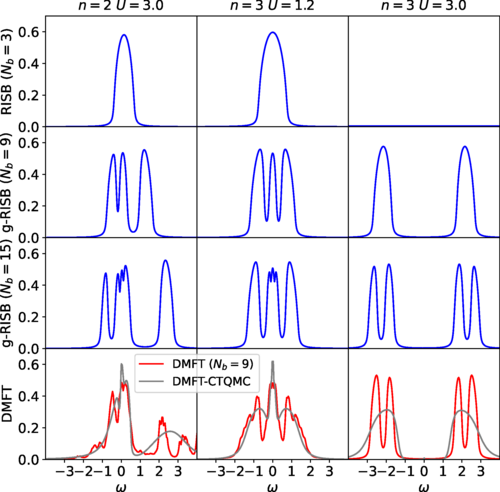
\includegraphics[width=0.85\textwidth]{hub_fig5.png}
    \end{column}
    \begin{column}{0.42\textwidth}
      \small
      3軌道 Hubbard，各列は異なるパラメータ\\
      行：RISB / g-RISB $N_b=9,15$ / DMFT

      \smallskip
      \begin{block}{\small 読み取り方}
        \footnotesize
        上から下へ $N_b$ を増やすと\\
        スペクトル関数が DMFT（最下行）\\
        に近づいていく
      \end{block}

      \smallskip
      \begin{alertblock}{\small 注意}
        \footnotesize
        エネルギー（$Z$, $E$）より\\
        スペクトル関数は収束が遅い\\
        → より大きな $N_b$ が必要
      \end{alertblock}
    \end{column}
  \end{columns}
\end{frame}

% ============================================================
\begin{frame}{付録C：Fermi 面の比較（Sr₂RuO₄）}
  \begin{columns}[T]
    \begin{column}{0.60\textwidth}
      \centering
      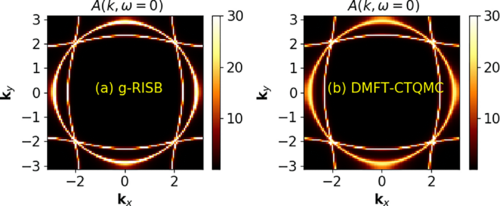
\includegraphics[width=\textwidth]{hub_fig8.png}
    \end{column}
    \begin{column}{0.37\textwidth}
      \small
      $\omega=0$ でのスペクトル関数\\
      $A(\mathbf{k}, \omega=0)$（Fermi 面）

      \smallskip
      \begin{block}{\small 結果}
        \footnotesize
        (a) g-RISB（$N_b=9$）\\
        (b) DMFT-CTQMC\\[4pt]
        Fermi 面の形がほぼ一致\\
        実材料でも g-RISB が有効
      \end{block}

      \smallskip
      {\footnotesize 実材料 Sr₂RuO₄\\
      $U=2.3$ eV，$J=0.4$ eV}
    \end{column}
  \end{columns}
\end{frame}

% ============================================================
\begin{frame}[shrink=18]{付録D：gGA の変分 Lagrangian}
  \begin{columns}[T]
    \begin{column}{0.54\textwidth}
      \small gGA は以下の Lagrangian を変分パラメータで停留させる：
      {\small
      \begin{align*}
        \mathcal{L} &=
          \frac{1}{\mathcal{N}}\langle\Psi_0|\hat{H}_\mathrm{qp}[\mathcal{R},\Lambda]|\Psi_0\rangle\\
          &+\langle\Phi|\hat{H}_\mathrm{emb}[\mathcal{D},\Lambda^c]|\Phi\rangle\\
          &-\sum_{a,b}(\Lambda_{ab}+\Lambda^c_{ab})\Delta_{ab}\\
          &+\sum_{c,a}\bigl(\mathcal{D}_a\mathcal{R}_c[\Delta(1-\Delta)]^{\frac{1}{2}}_{ca}+\mathrm{c.c.}\bigr)
      \end{align*}
      }

      \begin{block}{\small 変分パラメータ}
        \footnotesize
        $\mathcal{R}$：hopping 繰り込み行列\\
        $\mathcal{D}$：ghost との混成振幅\\
        $\Lambda, \Lambda^c$：bath エネルギー行列\\
        $\Delta$：ghost 占有行列
      \end{block}
    \end{column}

    \begin{column}{0.43\textwidth}
      \textbf{2つの補助系：}

      \smallskip
      \begin{block}{\small $|\Psi_0\rangle$（格子側）}
        \footnotesize
        $\hat{H}_\mathrm{qp}$ の基底状態\\
        ghost 空間の Slater 行列式\\
        $\to$ $\Delta_{ab}$ を与える
      \end{block}

      \smallskip
      \begin{block}{\small $|\Phi\rangle$（局所側）}
        \footnotesize
        $\hat{H}_\mathrm{emb}$ の基底状態\\
        物理サイト $+$ $B$ 個の ghost\\
        $\to$ 局所物理量を与える
      \end{block}

      \smallskip
      \begin{alertblock}{\small 停留条件}
        \footnotesize
        各パラメータへの微分 $= 0$\\
        $\to$ F1・F2 条件
      \end{alertblock}
    \end{column}
  \end{columns}
\end{frame}

% ============================================================
\begin{frame}[shrink=8]{付録E：計算設定}
  \small
  \begin{columns}[T]
    \begin{column}{0.50\textwidth}
      \textbf{モデルの詳細：}
      \begin{itemize}\itemsep1pt
        \item Bethe 格子，配位数 $z\to\infty$\\
          半円型 DOS，半幅 $D$（エネルギー単位）
        \item 半充填 $\langle\hat{n}_i\rangle=1$，常磁性相
        \item $U_i\simeq 0$（弱結合初期状態）$\to U_f$
      \end{itemize}

      \smallskip
      \textbf{gGA の設定：}
      \begin{itemize}\itemsep1pt
        \item ghost 軌道数 $B=1,2,3,5,7$（収束確認）
        \item 埋め込みH の次元：$4^{B+1}$\\
          （$B=3$：64次元，$B=7$：65536次元）
        \item 埋め込みH の基底状態：厳密対角化（ED）
      \end{itemize}
    \end{column}

    \begin{column}{0.47\textwidth}
      \textbf{初期条件：}
      \begin{itemize}\itemsep1pt
        \item $t<0$：$U_i$ での平衡 gGA を自己無撞着に解く
        \item $\Lambda=0$ ゲージで初期状態を準備
        \item $t=0$ で $U_i\to U_f$ に瞬時変化
      \end{itemize}

      \begin{block}{\footnotesize $\Lambda=0$ が一貫して成立する理由}
        \footnotesize
        $U_i\simeq 0$（非相互作用極限）では平衡解でも\\
        $\Lambda=0$ が自然に成立\\
        $\Rightarrow$ ゲージ変換なしに初期条件を準備可能
      \end{block}

      \smallskip
      \begin{block}{\footnotesize 時間積分}
        \footnotesize
        RKSUITE（adaptive Runge-Kutta）\\
        時間単位：$\hbar/D$\\
        $U_i\simeq0.05$：$U_i=0$ では\\
        $B\geq3$ で変分空間が縮退し\\
        自己無撞着計算が不安定になるため
      \end{block}

      \begin{alertblock}{\footnotesize コスト}
        \footnotesize
        各時刻で ED を解く必要なし\\
        $\Rightarrow$ ODE の右辺は代数演算のみ
      \end{alertblock}
    \end{column}
  \end{columns}
\end{frame}

% ============================================================
\begin{frame}{付録F：論文の実装 — $\Lambda=0$ ゲージ固定}
  \begin{columns}[T]
    \begin{column}{0.54\textwidth}
      論文（式(15)）は $\hat{H}_\mathrm{qp}$ に対して明示的に $\Lambda=0$ と設定：
      \begin{equation*}
        \hat{H}_\mathrm{qp}\big|_{\Lambda=0}
          =\sum_{a,b,\omega,\sigma}
            \epsilon_\omega\mathcal{R}_a\mathcal{R}_b^\dagger\,
            \eta^\dagger_{\omega a\sigma}\eta_{\omega b\sigma}
      \end{equation*}
      \textbf{時間発展する変分パラメータ：}
      $\mathbf{Y}=(\mathcal{R},\;\mathcal{D},\;\Delta,\;\Lambda^c,\;|\Phi\rangle)$

      \medskip
      \begin{block}{\small 正当化}
        \small $f_a\to\sum_b U_{ab}f_b$（$U\in\mathrm{U}(B)$）の下で\\
        $\hat{H}_\mathrm{qp}$ は不変，$\Lambda\to U\Lambda U^\dagger+(\text{補正})$\\
        $\Rightarrow$ $\Lambda=0$ はゲージ固定として正当化
      \end{block}
    \end{column}

    \begin{column}{0.43\textwidth}
      \begin{tikzpicture}[scale=0.9,
          box/.style={draw,rounded corners,
                      text width=3.6cm,align=center,inner sep=6pt}]
        \node[box,draw=myblue,fill=myblue!8](eq) at (0,1.5){
          \textbf{平衡 gGA}\\[3pt]
          \small $\Lambda$：自己無撞着に決定\\
          一般に $\Lambda\neq0$
        };
        \node[box,draw=mygreen,fill=mygreen!8](td) at (0,-0.8){
          \textbf{TD-gGA（論文）}\\[3pt]
          \small $\Lambda=0$ に固定\\
          ゲージ固定として処理
        };
        \draw[->,thick,myred,dashed](eq)--(td)
          node[midway,right,font=\footnotesize]{クエンチ};
      \end{tikzpicture}
    \end{column}
  \end{columns}
\end{frame}

% ============================================================
\begin{frame}{付録G：$\Lambda$ の取り扱いについて}
  \begin{alertblock}{核心的な疑問}
    平衡 gGA では $\Lambda\neq0$（自己無撞着に決定）\\
    TD-gGA（論文）では $\Lambda=0$ に固定 \quad \textbf{整合的か？}
  \end{alertblock}

  \smallskip
  \begin{columns}[T]
    \begin{column}{0.48\textwidth}
      \textbf{論文の立場：}
      \begin{itemize}
        \item $\Lambda$ は $\mathrm{U}(B)$ ゲージ自由度
        \item $\Lambda=0$ は常に選べるゲージ固定
        \item ゲージ不変な物理量は変わらない
      \end{itemize}
      \begin{block}{\small 初期条件}
        \small $U_i\simeq0$ の弱結合極限では\\
        $\Lambda\approx0$ が自然に成立
      \end{block}
    \end{column}

    \begin{column}{0.48\textwidth}
      \begin{alertblock}{\small オープンクエスチョン}
        \small $f_a\to U_{ab}f_b$ の下で\\
        $\mathcal{R},\mathcal{D},\Lambda^c$ がどう変換されるか\\
        の明示的な確認が必要
      \end{alertblock}
    \end{column}
  \end{columns}
\end{frame}

\end{document}
